\section{Appendix}
\appendix

\begin{frame}{Stimulate retina $\rightarrow$ control v4}{activate only one neuron of population with overlapping receptive fields}
    \begin{center}
    \adjincludegraphics[height=0.4\textheight,trim={0 0 {0.25\width} {0.46\height}},clip]{media/dicarlo_arch.jpg}
    \uncover<2>{
        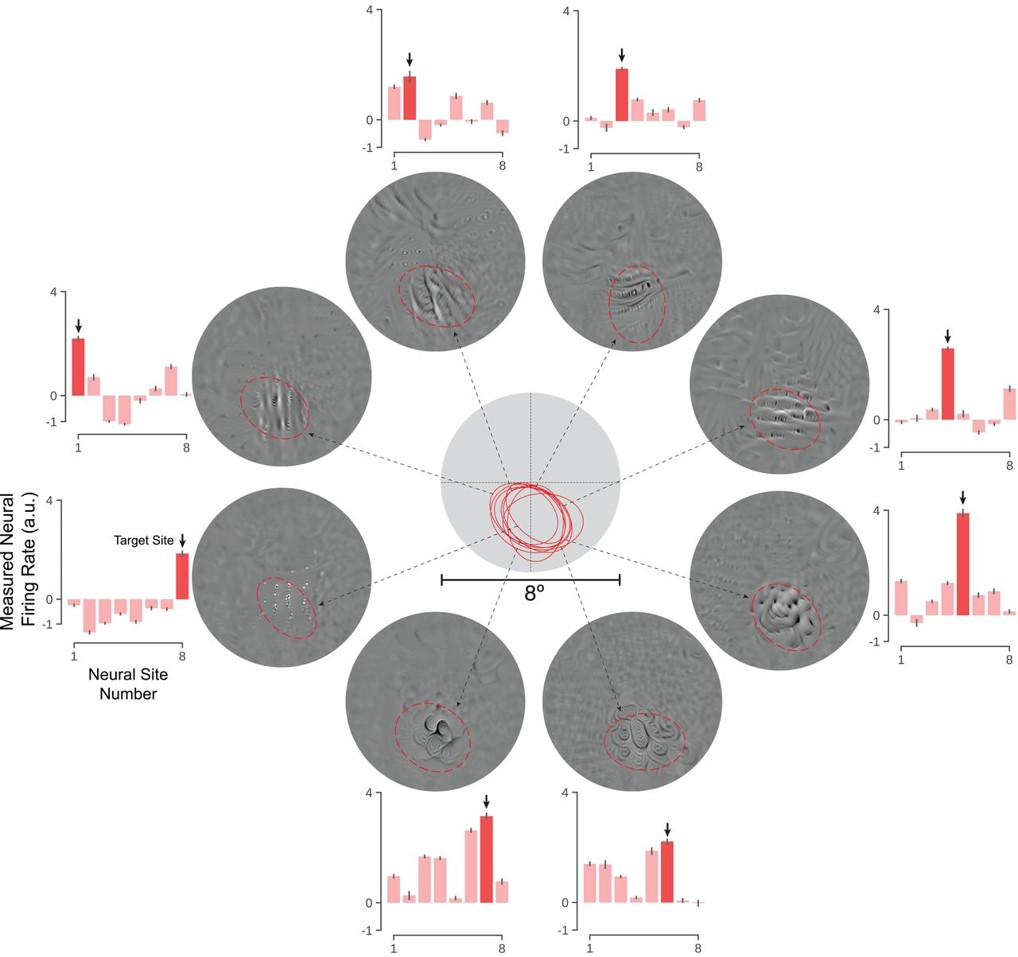
\includegraphics[height=0.5\textheight]{media/one-hot-control.jpg}
    }
    \nakedfootnote{Bashivan, Kar \& DiCarlo. \emph{Science}. 2019}
    \end{center}
    \note{Recently, some work has been done that reaches the Counterfactual rung: Deep Image Synthesis.

        train model on imagenet, regress conv layer to macaque V1 neurons. Use "Deep image synthesis" for one-hot population control. Example of counterfactual model--stim is very different from training! truly "imagined"}
\end{frame}{}

\begin{frame}{Linear Dynamical System with noise}
	\begin{align*}
		x_{t+1} = A x_t + \epsilon
	\end{align}
	\centering
	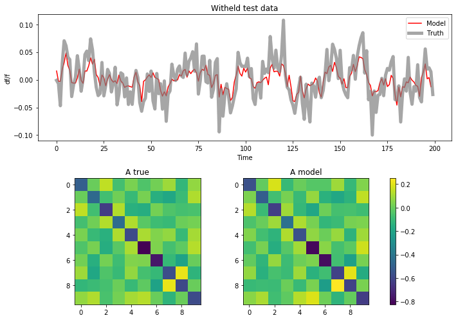
\includegraphics[height=0.8\textheight]{media/dcm_perfect}
\end{frame}

\begin{frame}{Reconstruction breaks down as noise increases}
	\centering
	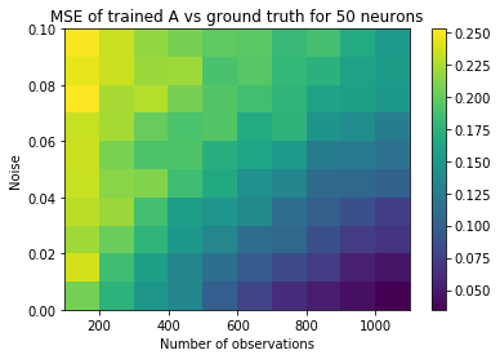
\includegraphics[width=0.8\textwidth]{media/dcm_fail}
\end{frame}


\begin{frame}{Whole-brain imaging at 200Hz}{exemplified by preliminary Extended Light Field Microscopy reconstruction}<handout:0>
				\centering
		    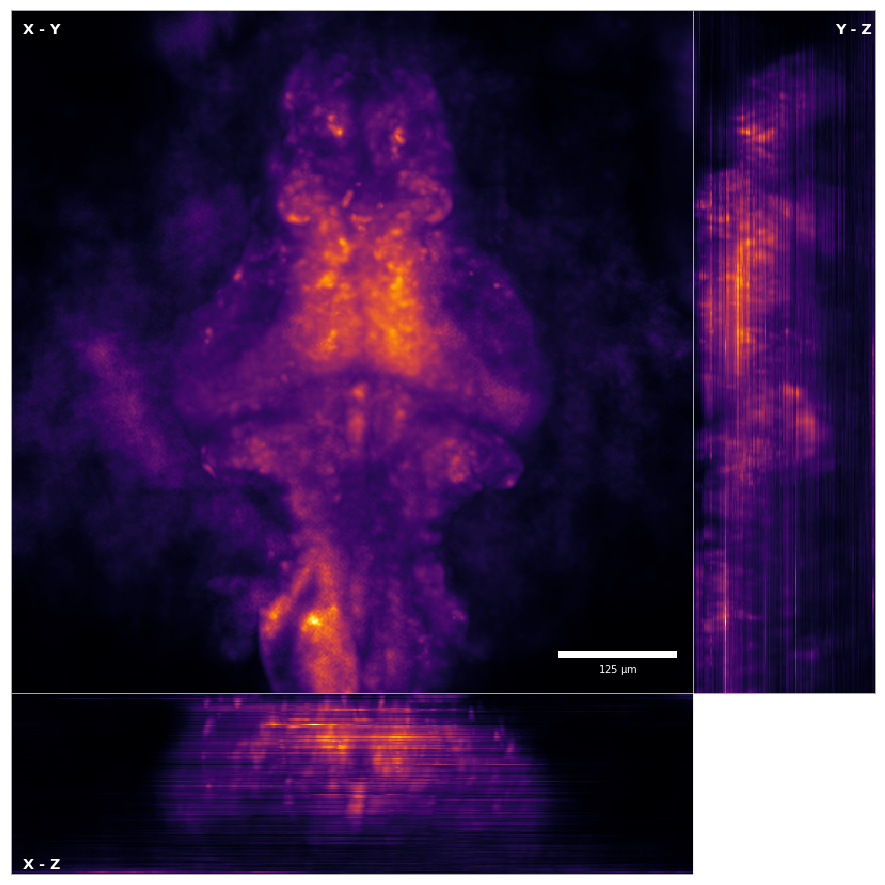
\includegraphics[height=0.8\textheight]{media/lfm.png}
        \linebreak
        1.4 TB/hr\nakedfootnote{Noah Young. \emph{unpublished}. 2019}
\end{frame}

\begin{frame}{ Learning physics from video prediction }{}<handout:0>
	\centering
	\movie[]{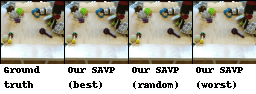
\includegraphics[height=0.28\textheight]{media/vid_pred_1.png}}{media/vid_pred_1.gif}
	\movie[]{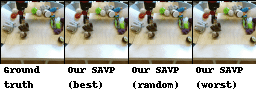
\includegraphics[height=0.28\textheight]{media/vid_pred_2.png}}{media/vid_pred_2.gif}
	\movie[]{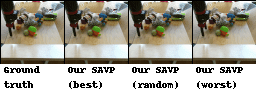
\includegraphics[height=0.28\textheight]{media/vid_pred_3.png}}{media/vid_pred_3.gif}
	% \movie[]{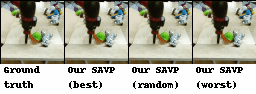
\includegraphics[width=\textwidth]{media/vid_pred_4.png}}{media/vid_pred_4.gif}
	\nakedfootnote{Lee, Zhang, et al. 2018}
\end{frame}

\begin{frame}{ Extracting principles from multiple fish }{}<handout:0>
    \centering
    \adjincludegraphics[width=0.9\textwidth,trim={{.05\width} {.7\height} {.2\width} {0.05\height}},clip]{media/hierarchical_bayes}\nakedfootnote{Koller \& Friedman. \emph{Probabilistic Graphical Models}. 2009.}
    % \adjincludegraphics[width=0.6\textwidth,trim={{.4\width} {.15\height} {0.05\width} {.25\height}},clip]{media/multi_fish_model.jpg}
    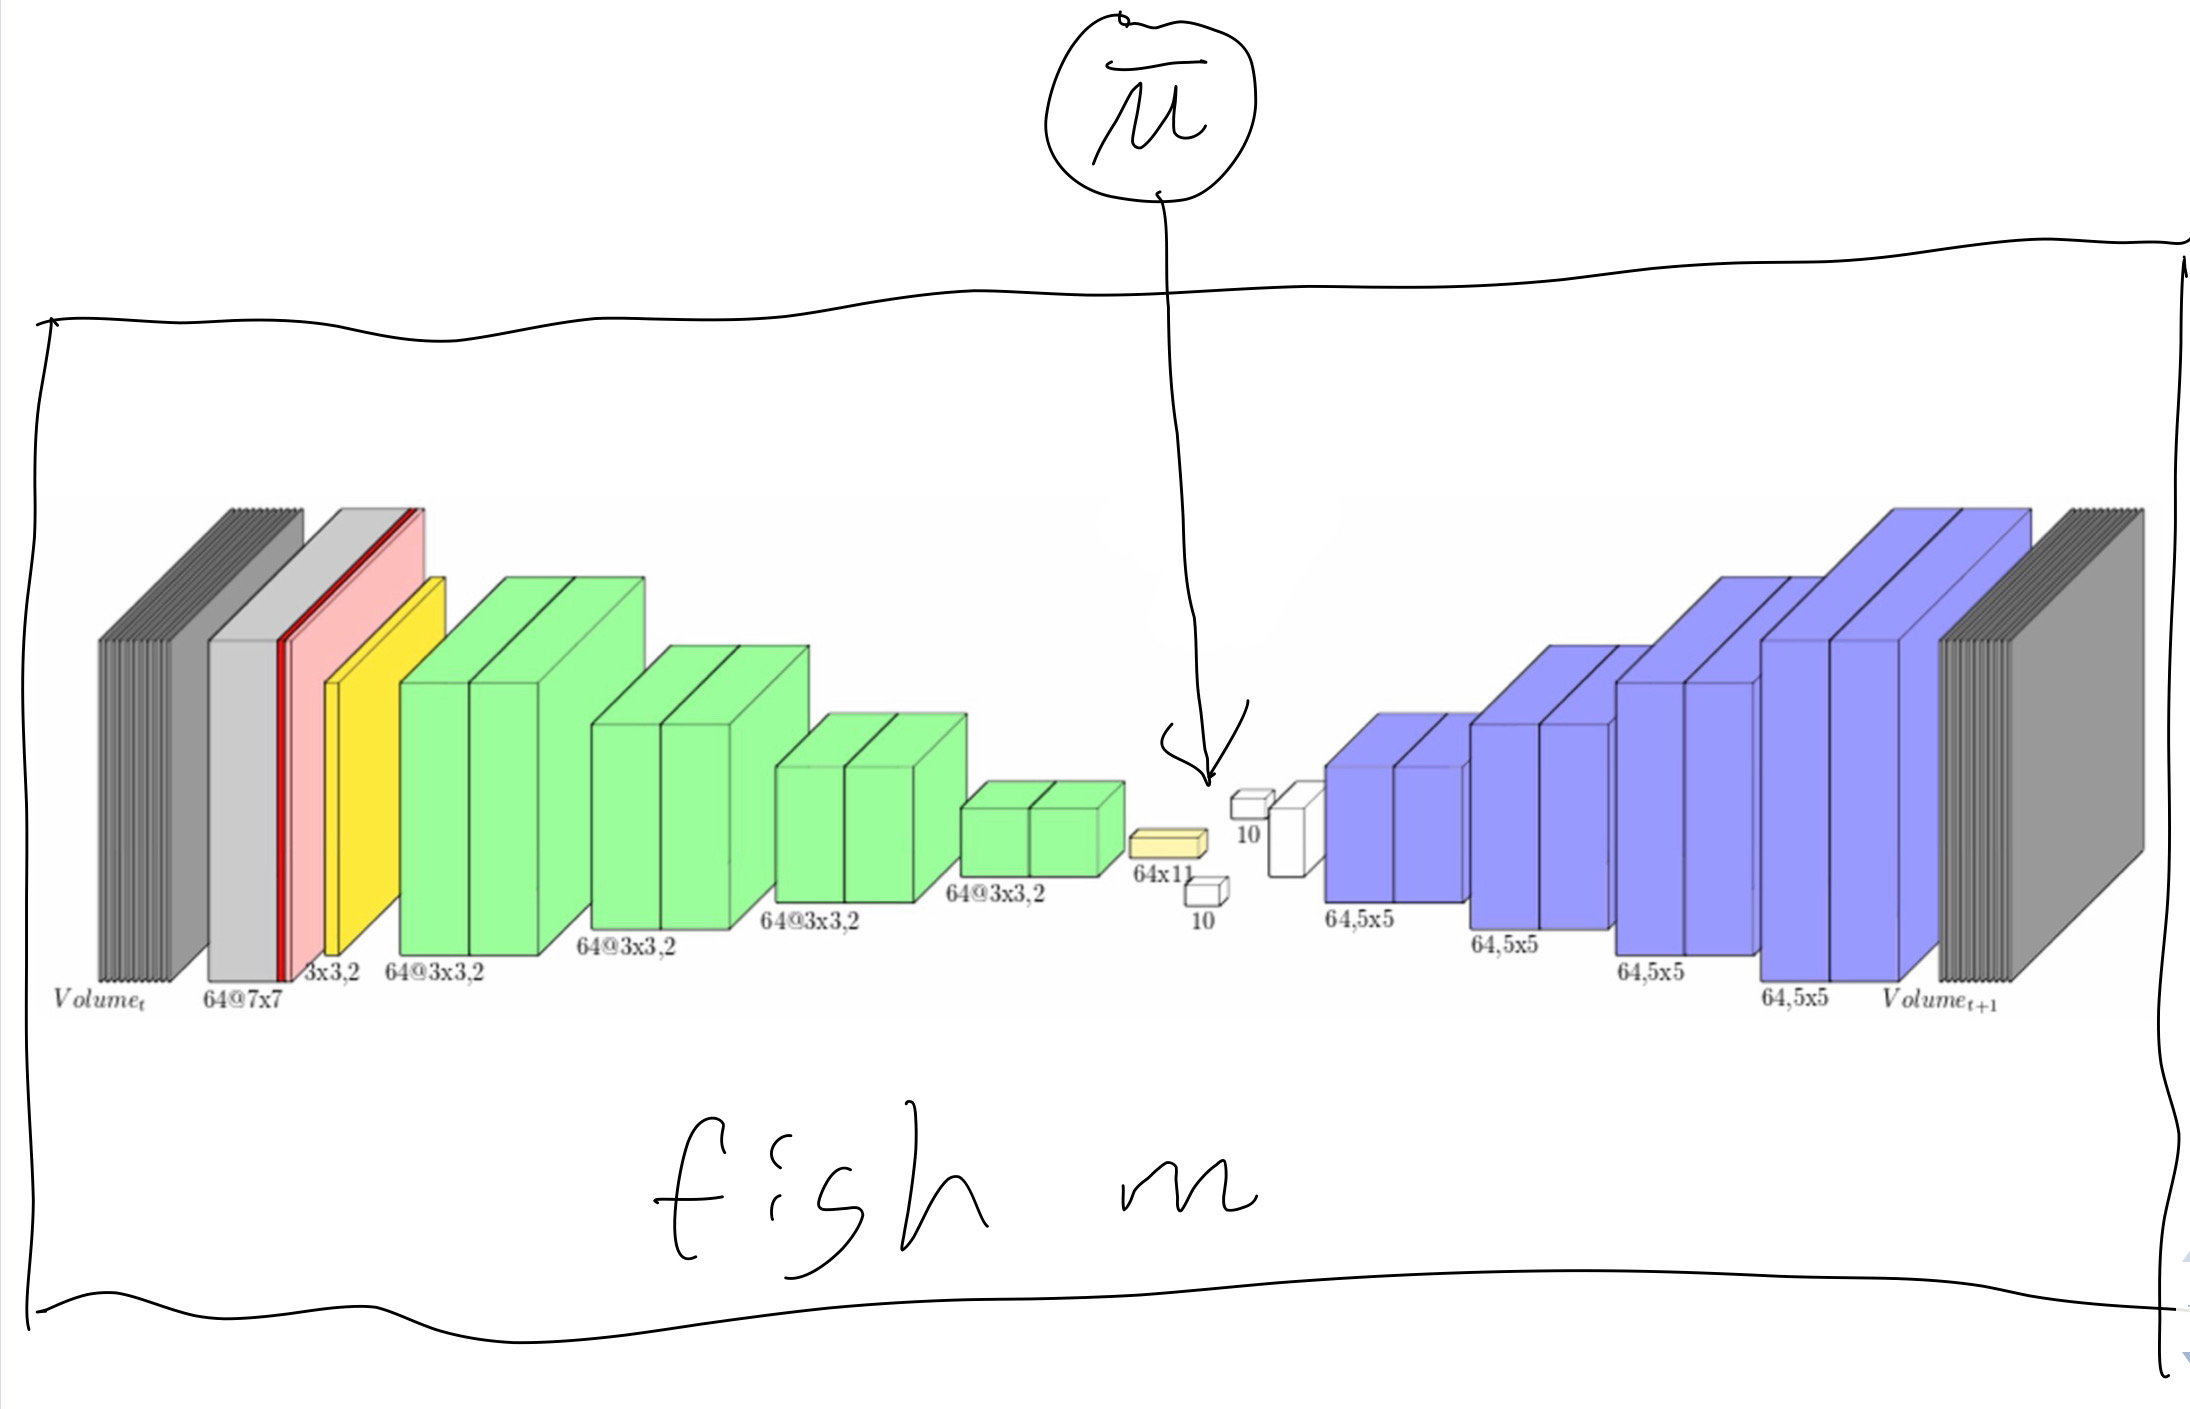
\includegraphics[height=0.5\textheight]{media/hierarchical-vp}
    \note{\textbf{placeholder} TODO: Talk about hierarchical bayes / extracting motifs / summarizing across multiple fish}
\end{frame}{}

\begin{frame}[t]{Modern deep learning toolkit}{}<handout:0>
	\begin{multicols}{2}
		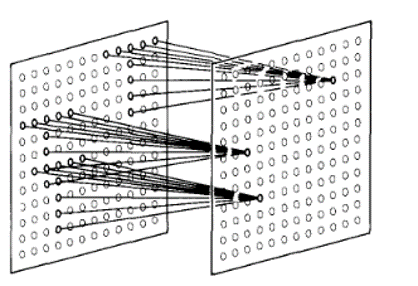
\includegraphics[height=0.32\textheight]{media/fukushima.png}
		Convolutional neural networks\textsuperscript{1}

		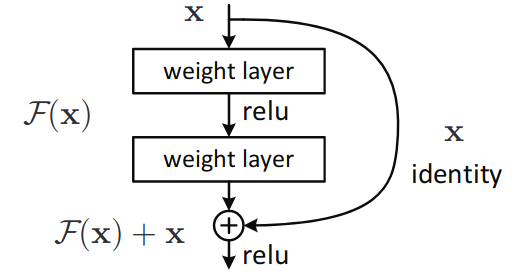
\includegraphics[height=0.32\textheight]{media/resblock.png}
		Deep residual structure \textsuperscript{2}

		\vfill\null\columnbreak

		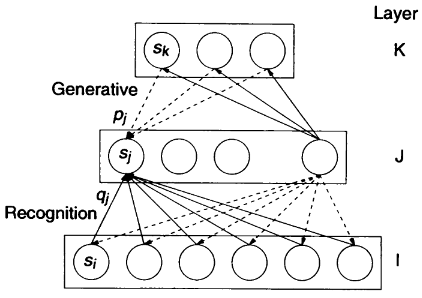
\includegraphics[height=0.35\textheight]{media/wakesleep.png}
		Variational Bayesian learning\textsuperscript{3}
		\note{A three-layer Helmholtz machine. The bottom layer represents the raw sensory inputs. When the units are driven bottom-up, the probability that $s_j = 1$ is $q_j$; when are driven top-down, the probability is $p_j$.
		}
		\\
		\makebox[0.5\textwidth][c]{%
			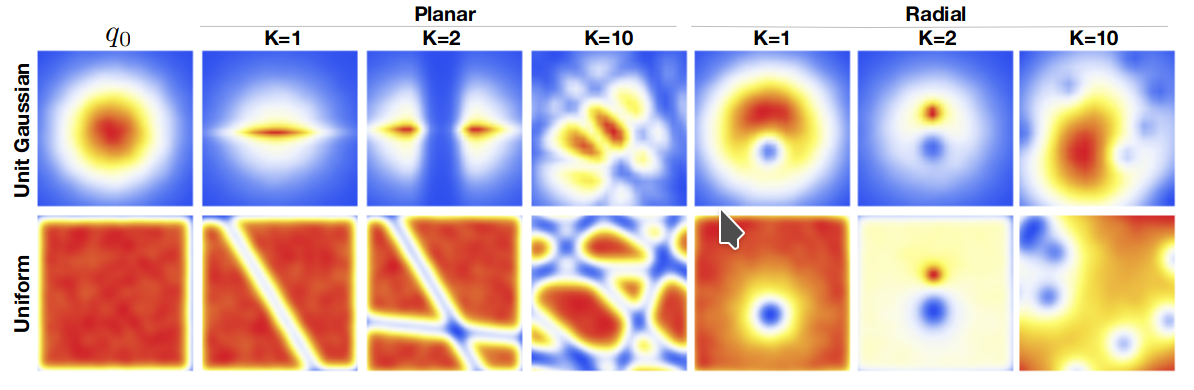
\includegraphics[width=0.6\textwidth]{media/normalizing_flow.png}
		}
		Normalizing flows
		\textsuperscript{4}
	\end{multicols}
	\vspace{-1cm}
	\nakedfootnote{Fukushima 1980 \textsuperscript{2}He et al 2015 \textsuperscript{3}Hinton et al 1995 \textsuperscript{4}Rezende\&Shaker 2016}
\end{frame}


\begin{frame}{Brain-computer interfaces}{``writing" into the brain}<handout:0>
	\centering
	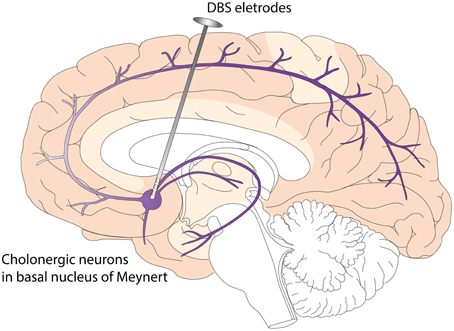
\includegraphics[height=0.4\textheight]{media/dbs}\nakedfootnote{Zhang \& Kim 2015 \uncover<2>{\emph{The Matrix} 1999.}}
	% 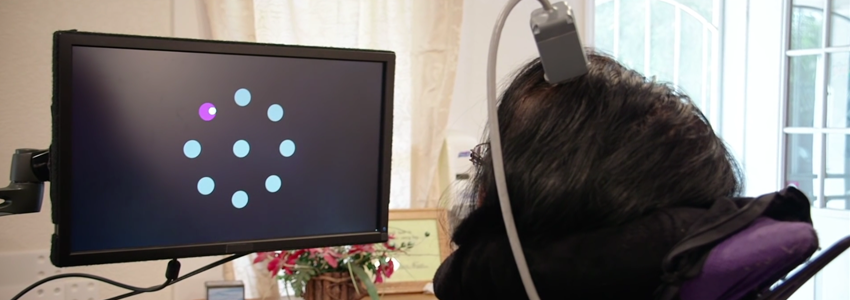
\includegraphics[width=0.6\textwidth]{media/bci}\nakedfootnote{https://youtu.be/9oka8hqsOzg}
	\uncover<2>{
		\movie[autostart]{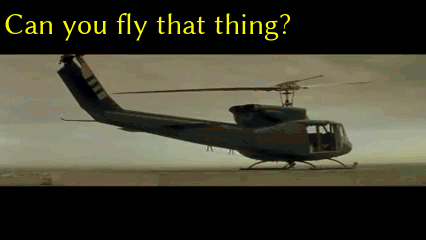
\includegraphics[height=0.5\textheight]{media/helicopter.png}}{media/helicopter.mp4}
	}
	\note<1>{Today's BCI often look like moving a cursor around a screen.}
	\note<2>{Pop media looks more like "downloading" how to fly a helicopter. We can't even conceptualize how such technology would work today.}
\end{frame}{}

\begin{frame}{ Canonical circuits }{}<handout:0>
    \centering
    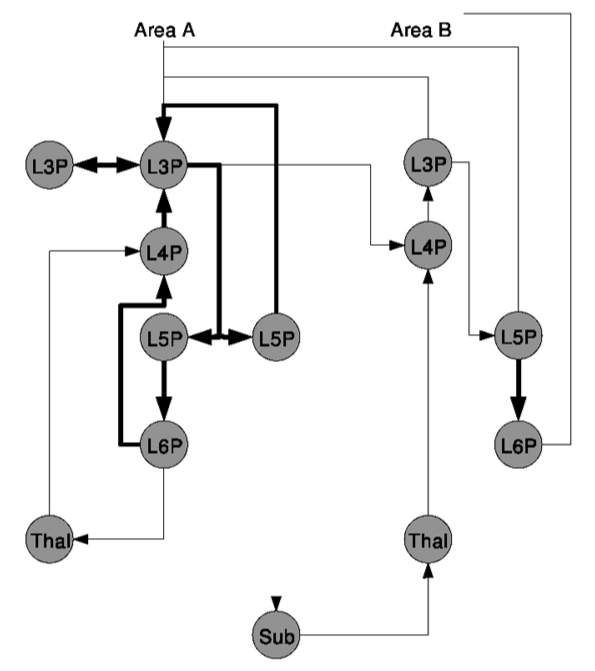
\includegraphics[height=0.8\textheight]{media/canonical}
\end{frame}

\begin{frame}{Bayesian optimization of latent space uncertainty}{multi-neuron stim}
    \movie[]{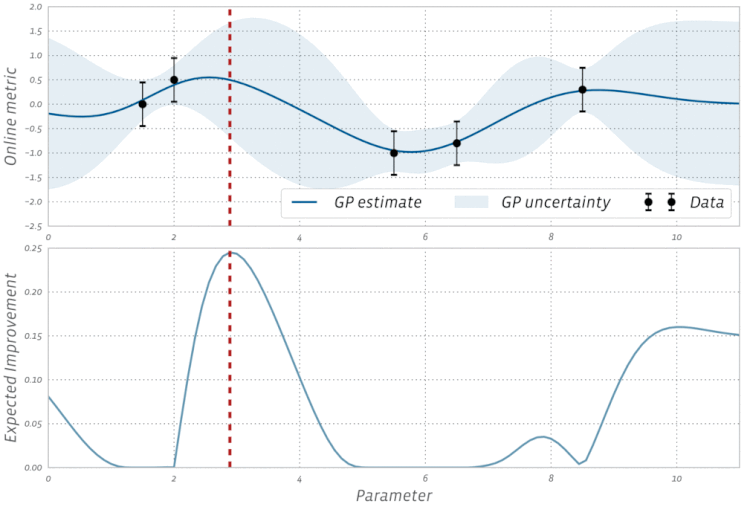
\includegraphics[height=0.85\textheight]{media/bayesian_opt.png}}{media/bayesian_opt.mp4}\nakedfootnote{github: Facebook/Ax}
    \note[item]{Note: this is a video.}
    \note[item]{Talk about bayesian nerual nets and distribution over network parameters}
    \note[item]{Alternatively, can formulate uncertainty in the latent space only.}
    \note[item]{Finding the best way to do this will be a concerted effort during PhD.}
    \note[item]{Pick stim that generates dynamics that reduce uncertainty.}
\end{frame}{}
